\minitoc

\section{Introduction}
\label{sec:testability:intro}
%\jgb{There was \cn both for the importance of building past snapshots, and for the importance of tests. I assume both things are evident enough, and don't need a citation. However, if you feel you can include a illustrating citation, please do.}

Reproducing (building) executable programs from the source code of past snapshots
%\patxi{Ojo, usa consistentemente snapshot o commit o change en la tesis. No recuerdo cómo está en el capítulo del emse al final}\michel{En este paper, el uso es consistente. En intro y related work se habla de snapshot. En la sección de definiciones, se introduce el commit como una snapshot del código fuente}
 of a project is fundamental for practitioners, to maintain old versions still in production, and for researchers, to study those old versions. 
To our knowledge, Tufano et al~\cite{tufano2017there} presented the most complete study on the compilability of past snapshots.
It analyzes all past snapshots for 100 Java projects of one organization (the Apache Software Foundation), determining how many of them could be built, and the main causes of failure in building. 
In these study, only 38\% of snapshots could be built, and almost all projects contained snapshots that could not be built (96\%).

However, not only the main executable program is of interest: both for maintenance and research reasons, building and executing tests of past snapshots is also important. 
For maintenance, because that allows developers to fix bugs/vulnerabilities~\cite{bartelsoftware} and backport functionality to some old version with some confidence~\cite{tian2017mining}, if all tests can be run and the result is succeeded, meaning the test did not find any misbehavior in the exercised part of the system. 
For researchers, because that allows for a more complete understanding of the project at those points in the past~\cite{santos2019mind}.

%Reproducing the state of every source code snapshot of a software project in the past has shown to be of interest, both for research and from a practical point of view \cn. 
%Although tests are an important part of software projects \cn, previous studies on reproducing the past have focused only on the compilability of the source code along project history. 

%\jgb{We could remove the next para, if we are short in space, and ensure we talk about it later, when discussing methods}

Nowadays, tests are so important to projects whose code is used in production, that they are usually an integral part of the process for accepting changes to the code base. In compiled languages such as Java, it is usual to run any new source code snapshot through a process which involves, in this order: compiling the main source code, compiling tests, running tests, and finally, building the package (e.g., a \texttt{jar} file) suitable for distribution. 
Only if all those steps succeed, the source code is deemed for production.

%In many projects, the Usually, building any snapshot involves several stages. For instance, when using the popular Maven tool for building Java projects, producing a package from a snapshot of a project requires following steps: i) compiling source code, ii) compiling tests, iii) running tests, and finally, iv) building the package (most commonly, a \texttt{jar} file) suitable for distribution. 

%In the same way that compilability is the ability of a project to make its snapshots buildable, testability is the ability of a project to ensure that the tests of each snapshot can be executed and pass successfully.

However, we are not aware of studies that systematically analyzed to which extent tests present in past snapshots can be built, and run with a result of success. Leveraging on the previous research on compilability of past snapshots, in this chapter we present a study that extends it having into account if testing of those past snapshots is still possible. 
Since there is no precedent on software testability in the past, we will start this chapter with a case study of project history testability to understand in depth how to measure it.
From this point on the term "compile" will be used instead of "build", for consistency with the previous section and because we will limit ourselves to using  projects written in Java (a compiled language), as we will see later on.
\michel{Yo aquí tengo muchas dudas, construir "build" y compilar "compile" no son  exactamente lo mismo. Yo entiendo que "build" es construir el paquete, y "compile" es compilar el código fuente. He cambiado la nomenclatura en la intro, pero por el momento no lo haré en el resto del paper.}
%\michel{Def: "A technique for detailed exploratory investigations, both prospectively and retrospectively, that attempt to understand and explain phenomenon or test theories, using primarily qualitative analysis"}
Our main aims are to study, for past snapshots of a project:

%Tufano et al. focused specifically on compiling source code. However, we argue that running the test suite is not only desirable, but mandatory for some use cases, like backporting bug fixes to previous versions or reproducing the past state of a system. That is why we decided to extend Tufano et al.'s paper, and focus on studying testability of past snapshots, with two main aims:

\textbf{(a)} The \textit{compilability} of tests: to which extent tests are still compilable from source code. 
This leads to the following research question:

\def \RQI{On how many snapshots of the change history can we compile tests?}
\def \RQII{On how many snapshots from the change history we can run all tests with a `success' result?}
% \def \RQIII{Is there any correlation between testability and other project characteristics such as size of the source code, length of the history of changes, or age?}

\textbf{RQ\textsubscript{1}}: ``\RQI''

\textbf{(b)} The \textit{testability} of the code: to which extent running tests of a snapshot result in success. 
This leads to the following research question:

\textbf{RQ\textsubscript{2}}: ``\RQII''

% \textbf{RQ\textsubscript{3}}: ``\RQIII''

We wanted to answer these questions in a manner that recognizes the diversity of software projects. For practical reasons, we considered only Java projects, which is already a reduction of scope. 
The projects have been selected from the ManySStuBs4J~\cite{karampatsis2020often} dataset.
% To avoid as much as possible further reduction, we decided to run three studies, all of them with the same method, but with different samples of projects. 
% We selected each sample so that its projects fulfill some common conditions (so that it is internally homogeneous, to some extent), but for each sample those conditions are different, trying to capture different kinds of projects. In all cases, we have focused on relatively large, mature projects used in production.

% The three samples of projects are based on (1) Apache projects studied by~\cite{tufano2017there} (compilability of past snapshots) (2) projects obtained through a search using the GitHub API by~\cite{maes2022revisiting} (a study extending the previous one), and (3) projects from ManySStuBs4J~\cite{karampatsis2020often}, a well-known dataset of Java projects used in mining software repositories.
The method we followed is in summary as follows: for each snapshot of each project, we automatically build its main code, its tests, and then we run tests whenever possible. 
We have performed this process for a total 86 different projects.

%For each project of each dataset, source and test code is built as preliminary steps for the execution of the tests, in order to adequately respond to the RQs.

%To define the testability of a snapshot, we will use the \textit{testable rate} of the test suite. 
%If a snapshot has a 100\% testable rate (all tests should build and result in \textit{success} when run) we will call it \textit{fully testable}.
To define the testability of a snapshot, we will verify if all its tests pass or fail, categorizing it as fully testable or not.
A fully testable snapshot would allow a developer to modify the code, and run all the tests again to check if the change breaks something.
% After running our studies, we can conclude that testability of past snapshots is relatively low: for 40.65\%\michel{Comprobar este valor} of all snapshots for which tests could be built, we obtained a \textit{success} result when running all the tests of each snapshot. 
The main result is that there is a large variation from project to project, with a few cases showing a high testability with all test succeeding in almost all their snapshots. 
\michel{Pocas conclusiones más veo con los resultados del capitulo.}
% For analyzing the results, we also provide a framework that permits to summarize in three metrics the main characteristics of a project with respect to testability of past snapshots. 

%In this paper we show in real projects how complicated it is to reproduce the building and test execution of a project in the past, extending the previous work of Tufano et.al.

%We have found projects where it is possible to reproduce these steps correctly. The tests are essential to ensure the correct functioning of the project. The execution of tests on past commits is crucial when we want to make changes on an old version of the project, ensuring that the code works as it did when it was written. 

The rest of the paper is structured as follows:
Section~\ref{sec:testability:methodology} presents the methodology used in the studies and defines the terminology. 
Section~\ref{sec:testability:case-study} shows the case study performed.
The results of applying the methodology are reported in Section~\ref{sec:testability:results}, while Section~\ref{sec:testability:analysis} offers a more detailed analysis of these results.
Section~\ref{sec:testability:discussion} discusses the results, and explores threats to their validity.
Finally, Section~\ref{sec:testability:conclusions} draws conclusions and presents further research.


\section{Definitions, data sources and methods}
\label{sec:testability:methodology}
%The objective of our study is to analyze the testability of open-source projects throughout their commit history.
%To check if the tests can be executed, two previous steps are necessary: i) compiling the source code, and ii) compiling the test code. 
%If either of the previous steps fail, no test execution study can be performed.
%Projects from three different datasets have been selected to carry out the same study on each of them.

Let us define some terminology used through this chapter, the collection of projects that we analyze, and the methods used for the analysis.
%In this section we define the terminology used, the datasets studied, the methodology applied and the metrics to be collected.

\subsection{Definitions}
\label{subsec:definitions}
%We derive the terminology used in this paper from Sulir et al.'s work~\cite{Sulir:2016:QSJ:3001878.3001882}. According to it, the build process of projects programmed with compilable languages consists of following steps:

In this subsection, we extend the terminology defined in Section~\ref{sec:buildability:definitions} to distinguish between main source code (code that is used to compile and build the executable) and testing code (code that verifies the correct behavior of the main source code, and will not be included in the package). 
We will also consider a further step consisting on running the tests, and collecting their results. 
The possible outcomes of a test execution are: \textbf{success}, if all test assertions are met, \textbf{failure}, if at least one of the assertions is not met, or \textbf{error}, if there is a problem in the test execution.
Therefore, considering the steps defined in Section~\ref{sec:buildability:definitions}, we would extend step 3 (\textit{execute the compiler to generate binary files from source code}) with 3 sub-steps:
\begin{inparaenum}[\bf(1)]
    \item \textit{compile the source code}
    \item \textit{compile the test code}, and
    \item \textit{execute the tests}.
\end{inparaenum}
With this in mind, we define:

%In particular, we define following concepts as follows:

\begin{itemize}
% \item \textbf{Commit}: a snapshot of the source code of a project, obtained by checking out a commit hash from git. Only commits on a given branch (usually \texttt{main} or \texttt{master}) will be considered, to keep history linear.
%    \item \textbf{Buildable source}: 
      %the ability of a version (commit) to be built successfully. We will consider the version as its source code and configuration files.
\item \textbf{Source-compilable}: a commit (snapshot) whose main source code can be successfully compiled. 
      % \item \textbf{Buildable test}: property of a version (commit) when its test code can be built successfully.
\item \textbf{Test-compilable}: a commit (snapshot) for which all tests can be successfully compiled (and has at least one test).
%\item \textbf{Testable Rate (for a given commit)}: ratio of success tests with respect to the total number of tests intended to run for that commit
\item \textbf{Fully Testable}: a commit (snapshot) for which all tests run with a success result.
      % property of a version (commit) when its tests can be executed with a successful result.

\end{itemize}

Based on this, we define the following metrics, that will characterize a project (for the considered git branch):
\begin{itemize}
    \item \textbf{Source Compilability}: ratio of \textit{source-compilable commits} with respect to the total number of commits.
    \item \textbf{Test Compilability}: ratio of \textit{test-compilable commits} with respect to the total number of commits.
    \item \textbf{Fully Testability}: ratio of \textit{fully testable commits} with respect to the total number of commits.
    % \item \textbf{Testability Rate\textsubscript{A}}: median of \textit{testable rate} for all commits in the project.
    % \item \textbf{Testability Rate\textsubscript{B}}: median of \textit{testable rate} for \textit{source-compilable commits} in the project.
    % \item \textbf{Testability Rate\textsubscript{T}}: median of \textit{testable rate} for \textit{test-compilable commits} in the project.
    % \item \textbf{Fully Testability\textsubscript{A}}: ratio of \textit{fully testable commits} with respect to the total number of commits.
    % \item \textbf{Fully Testability\textsubscript{B}}: ratio of \textit{fully testable commits} with respect to the number of \textit{source-compilable commits} of the project.
    % \item \textbf{Fully Testability\textsubscript{T}}: ratio of \textit{fully testable commits} with respect to the number of \textit{test-compilable commits} of the project.
\end{itemize}

% It should be noted that Sulir et al.~\cite{Sulir:2016:QSJ:3001878.3001882} use the term \textit{compilability} as the metric that measures how often the last commit of a project can be source compilable. In this paper, we will distinguish between \textit{Source Compilability} and \textit{Test Compilability}. We define \textbf{Source Compilability} as a metric with respect to the total number of commits of the project metric which measures how often these commits can be source compilable.
%Comparing with~\cite{Sulir:2016:QSJ:3001878.3001882}, it uses \textit{compilability} as the metric that measures how often the last commit of a project can be source compilable. In this paper, we will distinguish between \textit{Source Compilability} and \textit{Test Compilability}. We define \textbf{Source Compilability} as a metric with respect to the total number of commits of the project metric which measures how often these commits can be source compilable.
%On the other hand, we define \textbf{Test Compilability} as a metric with respect to the total number of source compilable commits of the project that measures how often these commits can be test compilable.

Each of these metrics tries to capture a \textit{ratio of progress} when we advance in the process towards running the tests. \textit{Source Compilability} informs on the ratio of snapshots that passed the first blocker: it only makes sense to test a snapshot if its main source could be built. This metric is quite similar to the one provided in previous chapter and by Tufano et.al~\cite{tufano2017there}, when studying compilability. From this point on, we introduce \textit{Test Compilability}, to determine the ratio that pass the next blocker: tests can be built.

%In this paper we define \textit{Fully Testability} at the project level (like with \textit{compilability}), although others have done it at the class or module level of an application~\cite{bruntink2006empirical}.
%Now, definitions for \textit{Testability} of a project are a bit trickier. 
% First, we consider as \textit{golden rule} for deciding if a snapshot is testable what developers would consider as ideal: that all tests run, and they all result in \textit{success}. 
% That would allow them to modify the code, and then run tests again to be sure that they are not having regressions. 
Thus, we define \textit{Testability} at the project level (as we did with \textit{compilability}), different from others who define it at the class or module level~\cite{bruntink2006empirical}.
% The \textbf{Testability Rate} of a project tells us what percentage of the tests we can run in the past, considering all the commits (\textbf{Testability Rate\textsubscript{A}}), all the commits where it is possible to build the source code (\textbf{Testability Rate\textsubscript{B}}) and all the commits commmits where we can build the tests (\textbf{Testability Rate\textsubscript{T}})

% In addition, processing the result of \textit{all} tests in binary form gives us information on whether a change in that commit would be supported by the tests. 
Processing the result of \textit{all} tests in binary form gives us information on whether a change in that commit would be supported by the tests. 
This way of characterizing a commit as \textit{Fully Testable} or not is also used in Continuous Integration (CI) systems to validate if a change (commit) can be integrated with the rest of the code of a project.
We define \textbf{Fully Testability} as a metric with respect to the total number of commits of the project metric which measures how often these commits can be fully testable.
% In this paper, we define \textbf{Fully Testability} as a metric with respect to the total number of commits of the project metric which measures how often these commits can be fully testable.

% As for the Testability Rate, we compute several ratios of testable commits, which provide different information about the \textbf{Fully Testability} of a project. 
% \textbf{Fully Testability\textsubscript{A}} gives the raw fraction of all commits that are testable, useful to determine if there are many snapshots where the \textit{all} tests pass. 
% \textbf{Fully Testability\textsubscript{B}} is the fraction of source-compilable commits where the \textit{all} tests pass, and \textbf{Fully Testability\textsubscript{T}} is the fraction of test-compilable commits where the \textit{all} tests pass. 
% Both provide information about how likely it is that tests pass if the main source code, or the tests, could be built.

%We have defined as \textit{"Golden Rule"} what a developer would consider a \textit{healthy} project: \textit{the source code must compile, the test code must compile and the tests must run successfully}.Tests are a fundamental part of a software project, they are necessary to check its proper performance. In previous versions of a project, they are especially useful to check how the project behaved. Under this definition, \textbf{Fully Testability\textsubscript{A}} is proposed, considering all the commits of a project.

%The results of the work of Tufano et al. show that one of the pre-requisites (source code compilability) is quite likely not to be fulfilled for a considerable number of commits. This has led us to propose \textbf{Fully Testability\textsubscript{B}}, which considers only those commits in which the source code can be built.

%Like source compilability, test compilability can prevent the completion of all the steps up to the execution of the test. Thus, we propose the \textbf{Fully Testability\textsubscript{T}}, as it is interesting to know how about the tests in those commits where it is possible to build \textit{both} the source code and the test code.

% We understand testability as a metric that conveys information about how often commits of a project are testable. We have considered the testabilitycwith respect to the total number of commits of the project~\textbf{Fully Testability\textsubscript{A}}, with respect to the source compilable commits~\textbf{Fully Testability\textsubscript{B}}, or with respect to the test compilable commits~\textbf{Fully Testability\textsubscript{T}}.

\subsection{Dataset}

%The selected dataset projects have been obtained from different sources, but all of them are Java projects whose build system is Maven. Maven is recognized as the most widely used system for project building and test execution in Java, and has been declared as a standard for Java projects \cn. 

We decided, mainly for practical reasons, to work with Java projects that are built with Maven. 
Even when this focus our study on a fraction of all software, still Java is a very popular language, with many mature projects used in production. 
Maven is recognized as the most widely used system for project building and test execution in Java, and as we have seen in the previous chapter, projects that use this technology are more likely to have a high Source Compilability.

However, we did not consider all Java-Maven projects. 
Android applications written in Java require dependencies on the Android~SDK, and have some peculiarities that make those projects different from \textit{regular} Maven projects. 
So, we discarded Android projects, following~\cite{Sulir:2016:QSJ:3001878.3001882} in this respect. 
We also discarded projects for which tests lasted too much to run until completion: we set a per-project limit of 60 real-time days for running tests for all snapshots.

%In addition, Android projects have been discarded due to the dependencies on the Android SDK. The building and execution of tests are especially delicate when it comes to Android projects and are very different from the experiment we want to carry out. Other authors~\cite{Sulir:2016:QSJ:3001878.3001882} also consider leaving out such projects when mining and building Java projects.

To carry out the experiment, we selected a subset of projects from the ManySStuBs4J dataset~\cite{karampatsis2020often}, a well-known set of 100 Java Maven projects used for Program Repair research.
From this dataset we discarded two projects that are no longer available in the public repository and 11 Android projects. 
In addition, one project has not been included as it has not finished the execution of its experiment, which has taken longer than any other project.
Therefore, 86 projects have been selected.

\subsection{Methods}
\label{subsec:methods}

After cloning the git repository of a project (from GitHub), we perform the following steps for each commit in their \textit{master/main} branch (the number of commits analyzed in each step can be seen in Figure~\ref{fig:methodology-process}):

\begin{enumerate}
    \item Checkout the commit.
    \item Compile the main source code by executing \textit{mvn clean compile -X}. If the command fails (the source build fails) the process stops. Otherwise, the commit is tagged as \textit{source compilable}.
    %In any case, the log of the command execution is saved.
    \item Build the test code by executing \textit{mvn test-compile}. If the command fails (the test build fails), or we detect there is no test in the snapshot, the process stops. Otherwise, the commit is tagged as \textit{test compilable}.
    %In any case, the log of the command execution is saved.
    \item Run the project tests by executing \textit{mvn test}, checking if all tests passed (labeling the commit as \textit{fully testable}).
      %Otherwise, it means that at least one test has failed or has had some kind of error. 
    %In any case, we will save the results of each test as Maven Surefire Reports~\footnote{https://maven.apache.org/surefire/maven-surefire-plugin/} in XML and TXT for each test case.
\end{enumerate}

%There are commits in some projects that do not have tests, and where executing the mentioned build and test execution commands does not result in a failure. Thus, only those commits that have at least one test will be considered as compilable/testable.

\begin{figure}[h!]
    \centering    
    \begin{tikzpicture}[node distance=1cm,every node/.style={fill=white, font=\sffamily}, align=center]
    \footnotesize
    % Specification of nodes (position, etc.)
    \node (total)             [large]                                         { 407,579 Commits};
    \node (buildable)         [large, below of=total]                         { 103,097 Source buildables commmits};
    \node (testBuildable)     [large, below of=buildable]                     { 93,925 Test buildables commits};
    \node (success)           [large, below of=testBuildable]                 { 40,540 Testable commits};

    \draw[-Latex]             (total) -- (buildable);
    \draw[-Latex]             (buildable) -- (testBuildable);
    \draw[-Latex]             (testBuildable) -- (success);

\end{tikzpicture}
    \caption{Study overview}
    \label{fig:methodology-process}
\end{figure}

%\subsection{Resulting metrics}
%\label{sec:metrics}

For each project, the following metrics are generated:

\begin{itemize}
    \item \textbf{Age:} Number of years since the first commit
    \item \textbf{LoC:} Number of lines of code of the project in its last commit
    \item \textbf{Total Commits:} Number of commits in the master branch
    \item \textbf{Source Buildable commits:} Number of commits that were source-compilable
    \item \textbf{Test compilable commits:} Number of commits that were test-compilable
    \item \textbf{Testable commits:} Number of testable commits
    %\item \textbf{\# commits w/ failed tests:} Number of commits where at least one of the tests failed without any error occurring.
    %\item \textbf{\# commits w/ errors tests:} Number of commits where at least one of the tests produced an error. \michel{Añadir las definiciones de eror y failed test} \mica{¿Omitir estas dos últimas métricas?}
\end{itemize}


As described in~\ref{subsec:definitions}, based on the last four of them we also generate for each project the metrics already defined at the beginning of this section: \textbf{Source Compilability}, \textbf{Test Compilability} and \textbf{Fully Testability}.
We include as well metrics such as project age, lines of code (LoC) and total commits because these are widely used when analyzing software projects~\cite{yamashita2015revisiting,mannan2016understanding,rosen2015commit}, and can bring an idea of the size of the projects. 

% \textbf{Testability Rate\textsubscript{A}}, \textbf{Testability Rate\textsubscript{B}}, \textbf{Testability Rate\textsubscript{T}},
% \textbf{Fully Testability\textsubscript{A}}, \textbf{Fully Testability\textsubscript{B}}, \textbf{Fully Testability\textsubscript{T}}.
%     \item \textbf{Source Compilability:} ratio of \textit{Buildable Commits} over \textit{Total commits}.
%     \item \textbf{Test Compilability:} ratio of \textit{Test compilable Commits} over \textit{Buildable Commits}.
%     \item \textbf{Fully Testability:} We consider three forms of testability, depending on the value on which it is calculated
%     \begin{itemize}
%         \item \textbf{Fully Testability\textsubscript{A}} percentage of \textit{Testable commits} over \textit{Total commits}.
%         \item \textbf{Fully Testability\textsubscript{B}} percentage of \textit{Testable commits} over \textit{Buildable Commits}.
%         \item \textbf{Fully Testability\textsubscript{T}} percentage of \textit{Testable commits} over \textit{Test compilable Commits}.
%     \end{itemize}
% \end{itemize}



\section{Case study}
\label{sec:testability:case-study}
In order to gain a deeper understanding of the testability of the commit history of software projects, we will conduct a case study, which is aimed to be an exploratory research with quantitative data analysis. 
In this case study, we will make an exploratory analysis of different projects, checking if the proposed testability metric (\textit{Fully Testability}) is able to represent the reality of the testability of the projects in all their history.
To quantitatively analyze the projects, we will use a graph per project that represents the results per commit of the steps described in the methodology. 

As can be seen in Figure~\ref{fig:projects-1}, each sub-figure represents the commit history of a project, where the X axis shows the commit number (0 for the first commit of the project, 1 for the second, etc.). On the Y axis we observe a stacked bar for each commit, with the height being the number of tests executed in that commit (denoted on the left Y-axis) and the colors (red, orange and green) indicating the results of each test (failure, error and success respectively). Additionally, the graph includes for each commit on the X-axis the number of lines of code (in blue) and test code (in purple) for that commit, with the values denoted on the right Y-axis.

%%%%%%%%%%%%%%%%%%%%%%%%%%%%%%%%%%%%%%%%%%%%%%%%%%%%%%%%%%%%%%%%%%%%%
%                            FIRST SET                              %
%%%%%%%%%%%%%%%%%%%%%%%%%%%%%%%%%%%%%%%%%%%%%%%%%%%%%%%%%%%%%%%%%%%%%

The first set of projects that we are going to study (Figure~\ref{fig:projects-1}) have been selected as a representative set of projects that, taking a look at their visual representation, it seems that it is possible to run the tests in the past in almost all their history.
Attending to the Source (Src) Compilability, Test Compilability and Fully Testability metrics of these projects (shown in Table~\ref{table:projects-1}), we observe that the results are in line with the charts.
For instance, in the sub-figure of the \textit{DiskLruCache} project there are commits with failures or errors in their tests, which affects to some extent its Fully Testability. 
Specifically, this metric drops to 70.58\%, which means that in almost 30\% of the commits, at least one test results in a failure or error.

\begin{figure}[!htb]
    \centering
    \begin{minipage}{.5\textwidth}
        \centering
        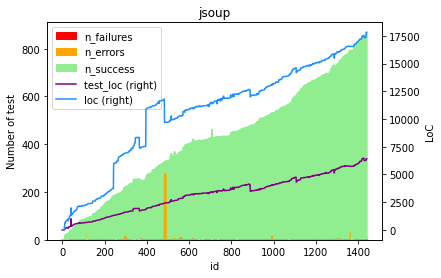
\includegraphics[width=\textwidth]{pages/02-Testability/images/projects/jsoup.png}
        \label{fig:jsoup}
    \end{minipage}%
    \begin{minipage}{.5\textwidth}
        \centering
        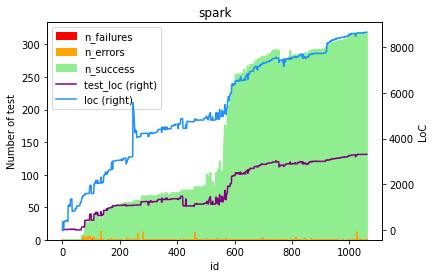
\includegraphics[width=\textwidth]{pages/02-Testability/images/projects/spark.png}
        \label{fig:spark}
    \end{minipage}
    \begin{minipage}{.5\textwidth}
        \centering
        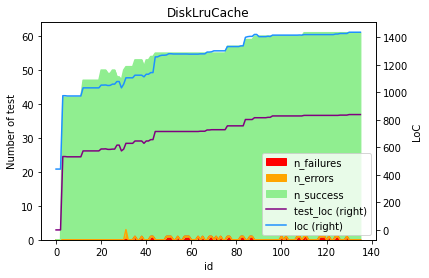
\includegraphics[width=\textwidth]{pages/02-Testability/images/projects/disklrucache.png}
        \label{fig:disklrucache}
    \end{minipage}%
    \caption{Set of projects 1: DiskLRUCache, Spark and JSoup}
    \label{fig:projects-1}
\end{figure}

\begin{table}[h!]
    \centering
    \resizebox{\textwidth}{!}{%
        \begin{tabular}{|r|r|r|r|}
        \hline
        \textbf{Project} & \textbf{Src Compilability}  & \textbf{Test Compilability} & \textbf{Fully Testability} \\ \hline
        jsoup            &  97.87\%                       & 97.29\%                      & 93.55\%                      \\ \hline
        spark            &  98.96\%                       & 92.84\%                      & 86.72\%                      \\ \hline
        DiskLruCache     &  100.00\%                      & 97.79\%                      & 70.58\%                      \\ \hline
        \end{tabular}
    }
    \caption{Metrics of set of projects 1: JSoup, Spark and DiskLRUCache}
    \label{table:projects-1}
\end{table}

%%%%%%%%%%%%%%%%%%%%%%%%%%%%%%%%%%%%%%%%%%%%%%%%%%%%%%%%%%%%%%%%%%%%%
%                           SECOND SET                              %
%%%%%%%%%%%%%%%%%%%%%%%%%%%%%%%%%%%%%%%%%%%%%%%%%%%%%%%%%%%%%%%%%%%%%

The second set of project that we are going to study (Figure~\ref{fig:projects-2}) have been selected as a representative set of projects that, taking a look at their visual representation, it seems that it is possible to run the tests in the past in almost all their history, although in some of them we find multiple commits where failures or errors are located.
However, if we look again at the Fully Testability values (Table~\ref{table:projects-2}), we find that their values are surprisingly low. 
For example, the \textit{Checkstyle} project, despite the fact that a portion of its commits at the beginning of the project are not compilable, the figure seems to indicate that almost all of its tests pass. 
Its low Fully Testability value is due to a few tests fail\patxi{failing consistently (in the order of 10 out of 1000)?}\michel{Como en la figura se muestra la cantidad de test verdes/rojos que hay, se puede apreciar que en la mayoria de commits el \% es muy bajo, menos de 10 por cada 1000} along the project history.
% \michel{He vuelto a mirar muy en detalle, parece que al re-ejecutarlo han cambiado un poco los resultados. En un párrafo no puedo comentarte exacatemente lo que he encontrado. Tengo que enseñarte las tablas y comentarte. Rápidamente puedo decir que en este proyecto solo pasan los test en el 0.01\% de los commtis (81). En la mayoria de commits, un porcentaje muy bajo de test fallan. En un commit en concreto fallan 17 test, pero en los demás es menos de 10 (con +1000 test). Hay test que fallan en todos los commits, pero no son muchos (17 test únicos). Hay un par de test más que fallan en muy pocos commits. Para ver los logs de porqué fallan esos test tengo que bajarme los resultados de Minio y descomprimirlos, por lo que me gustaría comentarlo antes}
The other two projects expose a similar behavior, in the case of \textit{HikariCP} the failures are more visible in the graph (there are more tests per commit resulting in failures or errors) despite having the highest Fully Testability value of this set.

\begin{figure}[!htb]
    \centering
    \begin{minipage}{.5\linewidth}
        \centering
        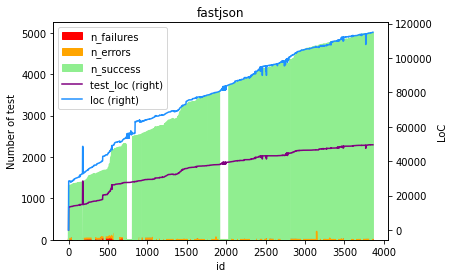
\includegraphics[width=\textwidth]{pages/02-Testability/images/projects/fastjson.png}
        \label{fig:fastjson}
    \end{minipage}%
    \begin{minipage}{.5\linewidth}
        \centering
        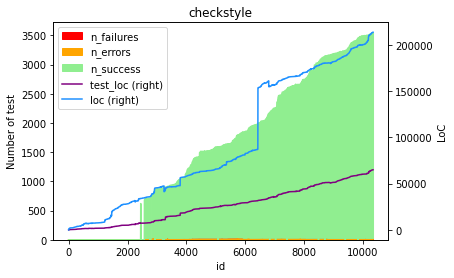
\includegraphics[width=\textwidth]{pages/02-Testability/images/projects/checkstyle.png}
        \label{fig:checkstyle}
    \end{minipage}
    \begin{minipage}{.5\linewidth}
        \centering
        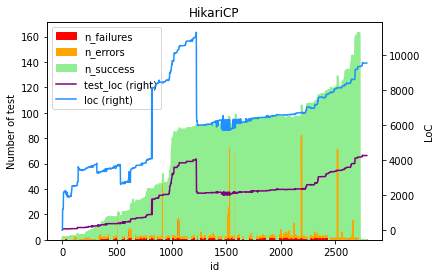
\includegraphics[width=\textwidth]{pages/02-Testability/images/projects/hikari.png}
        \label{fig:hikari}
    \end{minipage}%
    \caption{Set of projects 2: Fastjson, Checkstyle and HikariCP}
    \label{fig:projects-2}
\end{figure}

\begin{table}[h!]
    \centering
    \resizebox{\textwidth}{!}{%
        \begin{tabular}{|r|r|r|r|}
        \hline
        \textbf{Project} & \textbf{Src Compilability} & \textbf{Test Compilability} & \textbf{Fully Testability} \\ \hline
        HikariCP         &  96.02\%                      & 95.22\%                      & 16.92\%                      \\ \hline
        Checkstyle       &  77.72\%                      & 74.35\%                      & 0.78\%                      \\ \hline
        Fastjson         &  94.25\%                      & 88.35\%                      & 0.00\%                      \\ \hline
        \end{tabular}
        }
    \caption{Metrics of set of projects 1: Fastjson, Checkstyle and HikariCP}
    \label{table:projects-2}
\end{table}

Considering the above-mentioned results, Fully Testability is a very restrictive metric, as soon as a single test does not pass consistently in several commits, it drastically reduces the value of the metric. 
We can consider that we are missing information about the real testability of the project.
From the point of view of a practitioner or a researcher who needs to add a change to a past version and has to evaluate if the tests allow him to be sure not to introduce any regression in the code, knowing that in a commit 99.99\% of the tests pass may be enough.
This happened in the case of the \textit{Checkstyle} project, where there are commits with 3506 tests but only 1 fails.
\patxi{Esta frase es muy larga pero no sé cómo partirla.}
\michel{He sacado el texto del parentesis (el ejemplo) como una nueva frase para aligerlo un poco.}

Following this discussion, we propose a new and less restrictive way of measuring testability, which allows us to capture the information in a non-binary way. 
Instead of using a binary value (a commit is either Fully Testable or not) we will use a ratio. 
Hence, a commit has a \textbf{Testable Rate}, defined as the ratio of success tests with respect to the total number of tests run for that commit.
For a project, we would obtain the \textbf{Testability Rate} as the mean of the Testable Rate value of all commits in the history.

Table~\ref{table:projects-2-with-testability-rate} shows the Testability Rate results for the second set of projects.
This new metric reflects a higher testability value for this set of projects, which is in line with the reality of the tests executed.

\begin{table}[h!]
    \centering
    \resizebox{\textwidth}{!}{%
        \begin{tabular}{|r|r|r|r|r|}
        \hline
        \textbf{Project} & \multicolumn{1}{c|}{\textbf{\begin{tabular}[c]{@{}c@{}}Src \\ Compilability\end{tabular}}} & \multicolumn{1}{c|}{\textbf{\begin{tabular}[c]{@{}c@{}}Test \\ Compilability\end{tabular}}} & \multicolumn{1}{c|}{\textbf{\begin{tabular}[c]{@{}c@{}}Fully\\ Testability\end{tabular}}} & \multicolumn{1}{c|}{\textbf{\begin{tabular}[c]{@{}c@{}}Testability\\ Rate\end{tabular}}} \\ \hline
        HikariCP         &  96.02\%                      & 95.22\%                      & 16.92\%                      & 88.76\%                     \\ \hline
        checkstyle       &  77.72\%                      & 74.35\%                      & 0.78\%                       & 74.22\%                     \\ \hline
        fastjson         &  94.25\%                      & 88.35\%                      & 0.00\%                       & 87.80\%                     \\ \hline
        \end{tabular}
    }
    \caption{Metrics of set of projects 1: Fastjson, Checkstyle and HikariCP (including the new Testability Rate metric)}
    \label{table:projects-2-with-testability-rate}
\end{table}

%%%%%%%%%%%%%%%%%%%%%%%%%%%%%%%%%%%%%%%%%%%%%%%%%%%%%%%%%%%%%%%%%%%%%
%                            THIRD SET                              %
%%%%%%%%%%%%%%%%%%%%%%%%%%%%%%%%%%%%%%%%%%%%%%%%%%%%%%%%%%%%%%%%%%%%%

The third set of projects is shown in Figure~\ref{fig:projects-3}. 
In this case, we have chosen projects that appear to be very testable but only in a part of their history (due to problems in compiling the source code or test code).
Table~\ref{table:projects-3} shows the testability values for these projects. 

\begin{figure}[!htb]
    \centering
    \begin{minipage}{.5\linewidth}
        \centering
        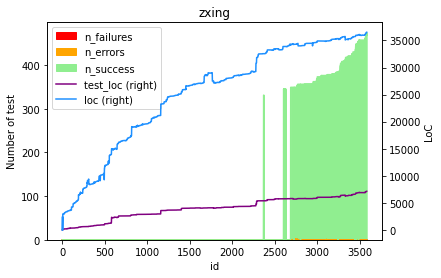
\includegraphics[width=\textwidth]{pages/02-Testability/images/projects/zxing.png}
        \label{fig:zxing}
    \end{minipage}%
    \begin{minipage}{.5\linewidth}
        \centering
        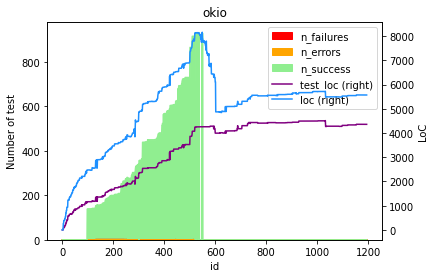
\includegraphics[width=\textwidth]{pages/02-Testability/images/projects/okio.png}
        \label{fig:okio}
    \end{minipage}
    \begin{minipage}{.5\linewidth}
        \centering
        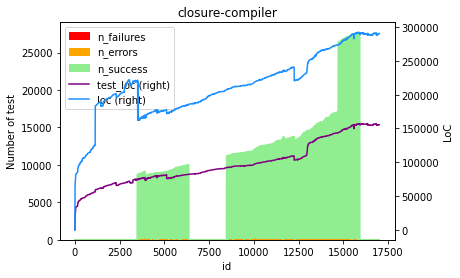
\includegraphics[width=\textwidth]{pages/02-Testability/images/projects/closure.png}
        \label{fig:closure-compiler}
    \end{minipage}%
    \caption{Set of projects 3: Zxing, Okio and Closure}
    \label{fig:projects-3}
\end{figure}

\begin{table}[h!]
    \centering
    \resizebox{\textwidth}{!}{%
        \begin{tabular}{|r|r|r|r|r|}
            \hline
            \textbf{Project} & \multicolumn{1}{c|}{\textbf{\begin{tabular}[c]{@{}c@{}}Src \\ Compilability\end{tabular}}} & \multicolumn{1}{c|}{\textbf{\begin{tabular}[c]{@{}c@{}}Test \\ Compilability\end{tabular}}} & \multicolumn{1}{c|}{\textbf{\begin{tabular}[c]{@{}c@{}}Fully\\ Testability\end{tabular}}} & \multicolumn{1}{c|}{\textbf{\begin{tabular}[c]{@{}c@{}}Testability\\ Rate\end{tabular}}} \\ \hline
            okio             & 36.65 & 36.06\%                      & 26.27\%                       & 36.01\%                     \\ \hline
            closure          & 60.18 & 59.84\%                      & 55.81\%                       & 59.84\%                     \\ \hline
            zxing            & 25.47 & 25.39\%                      & 24.80\%                       & 25.38\%                     \\ \hline
        \end{tabular}
    }
    \vspace*{0.5cm}
    \captionof{table}{Metrics of set of projects 3: Zxing, Okio and Closure}
    \label{table:projects-3}
\end{table}

These projects are characterized by a low Test Compilability. 
The Test Compilability metric is greatly affected by Source Compilability; if the code does not compile, the tests cannot be compiled. 
The reasons why source code cannot be compiled have been studied in previous chapter and in previous work~\cite{tufano2017there,Sulir:2016:QSJ:3001878.3001882}, and are caused mainly because of the impossibility to reproduce the context and retrieve the dependencies of a particular commit. 
For the okio, closure and zxing projects, the Source Compilability values are very close to Test Compilability values.
So, we can state that in these projects, if the source code compiles, in most cases the test code compiles as well. 
We can reflect this in a new metric: Test Compilability\textsubscript{S}, the ratio of test-compilable commits with respect to the source-compilable commits.
The Test Compilability metric, when calculated considering all commits in the project history, is renamed to Test Compilability\textsubscript{A}.
Table~\ref{table:projects-3-B} shows the values of these two variants of Test Compilability, in addition to the Source Compilability values mentioned above.


\begin{table}[h!]
    \centering
    \resizebox{\textwidth}{!}{%
        \begin{tabular}{|r|r|r|r|r|r|}
        \hline
        \multicolumn{1}{|c|}{\textbf{Project}} & \multicolumn{1}{c|}{\textbf{\begin{tabular}[c]{@{}c@{}}Src \\ Compilability\end{tabular}}} & \multicolumn{1}{c|}{\textbf{\begin{tabular}[c]{@{}c@{}}Test \\ Compilability\textsubscript{A}\end{tabular}}} & \multicolumn{1}{c|}{\textbf{\begin{tabular}[c]{@{}c@{}}Test \\ Compilability\textsubscript{S}\end{tabular}}} & \multicolumn{1}{c|}{\textbf{\begin{tabular}[c]{@{}c@{}}Fully\\ Testability\end{tabular}}} & \multicolumn{1}{c|}{\textbf{\begin{tabular}[c]{@{}c@{}}Testability\\ Rate\end{tabular}}} \\ \hline
        okio                                   & 36.65\%                                                                                        & 36.07\%                                                                                         & 98.40\%                                                                                         & 26.28\%                                                                                     & 36.02\%                                         \\ \hline
        closure                                & 60.18\%                                                                                        & 59.84\%                                                                                         & 99.43\%                                                                                         & 55.82\%                                                                                     & 59.84\%                                         \\ \hline
        zxing                                  & 25.47\%                                                                                        & 25.39\%                                                                                         & 99.67\%                                                                                         & 24.80\%                                                                                     & 25.39\%                                         \\ \hline
        \end{tabular}
    }
    \captionof{table}{Extended metrics of set of projects 3: Zxing, Okio and Closure}
    \label{table:projects-3-B}
\end{table}

Following the idea of focusing on those commits where we can compile the test code, we should consider that it is possible that the commits that do not compile, never did and therefore their testability information is not useful to us.
% Once again we find that the testability metrics do not provide all the information. 
% When we cannot compile source code or test code, we lose testability information. 
For projects such as those in set 3, the testability of the commits where we can compile the tests gives us valuable information that neither the Fully Testability nor the Testability Rate capture, as both metrics are calculated from all commits in the history of the project.

To capture the testability of Test Compilable commits we define the following metrics:
\begin{itemize}
    \item \textbf{Testability Rate\textsubscript{T}}: mean of \textit{testable rate} for \textit{test-compilable commits} in the project.
    \item \textbf{Fully Testability\textsubscript{T}}: ratio of \textit{fully testable commits} with respect to the number of \textit{test-compilable commits} of the project.
\end{itemize}
The Fully Testability and Testability Rate metrics, when calculated considering all the commits in the history, are renamed Fully Testability\textsubscript{A} and Testability Rate\textsubscript{A}.

In Table~\ref{table:projects-3-with-flavor-testability-rate} we include the new metrics defined for the third set of projects. 
We note that for all 3 projects, the new metrics more closely capture the testability of the commits we can compile.
The Fully Testability\textsubscript{T} shows us that for those commits where we can compile the tests, a high percentage can run all their tests with a success result. For this same set of commits, the Testability Rate\textsubscript{T} shows us values close to 100\%; almost all of the tests in these commits offer a success result.

\begin{table*}[h!]
    \centering
    \resizebox{\textwidth}{!}{%
        \begin{tabular}{|r|r|r|r|r|r|r|r|}
            \hline
            \rH{Project} & \rH{Src\\ Compilability} & \rH{Test\\ Compilability\textsubscript{A}} & \rH{Test\\ Compilability\textsubscript{S}} & \rH{Fully\\Testability\textsubscript{A}} & \rH{Fully\\Testability\textsubscript{T}} & \rH{Testability\\Rate\textsubscript{A}} & \rH{Testability\\Rate\textsubscript{T}} \\ \hline
            okio             & 36.65\%                        & 36.07\%                         & 98.40\%                         & 26.28\%                        & 72.85\%                        & 36.02\%                       & 99.86\%                       \\ \hline
            closure          & 60.18\%                        & 59.84\%                         & 99.43\%                         & 55.82\%                        & 93.27\%                        & 59.84\%                       & 99.99\%                       \\ \hline
            zxing            & 25.47\%                        & 25.39\%                         & 99.67\%                         & 24.80\%                        & 97.69\%                        & 25.39\%                       & 100.00\%                      \\ \hline
        \end{tabular}
    }
    \caption{Extended metrics of set of projects 3: Zxing, Okio and Closure (including the new Testability Rate\textsubscript{T} and Fully Testability\textsubscript{T} metrics)}
    \label{table:projects-3-with-flavor-testability-rate}
\end{table*}

%\patxi{Podría ser interesante incluir también o analizar los del conjunto 1, para dar una idea de la robustez de esta métrica: ¿sigue manteniéndose alta en el primer conjunto de proyectos y refleja por tanto lo que queremos?}
%\michel{Temo sobrecargar esta sección de tablas. Mi impresión es que las métricas son esperables teniendo en cuenta los razonamientos que hemos hecho, no aportan nada nuevo.}

\def \RQIII{How many tests of a snapshot can be run with a `success' result?}

This case study helped us to define metrics that better describe a project's stability. These new metrics lead to a new research question: 

\textbf{RQ\textsubscript{3}}: ``\RQIII''
\michel{Habría quedar una vuelta a la pregunta}
\patxi{Yo diría: For those commits of a project on which tests compile, how many of them can be run with a success result?}
\michel{To discuss: Ojo cuidado, que la pregunta deberia ser para todos los commits, no solo para los compilables. (No lo digo yo, este comentario lo ha generado Copilot :D). Solo los compilables es la TestabilityRate_T}

\section{Experimental results}
\label{sec:testability:results}
Once we performed our case study and determined the metrics that might better represent the projects, in this section we resort to describe the results in detail using the metrics defined in the previous section.

After running the experiment, we detected 20 projects in which not a single test was run on any commit in the history. 
The learning-spark project does not contain any tests in any commit of its history. 
The Mycat-Server project has a dependency on software that must be installed on the machine for it to be compiled (therefore its Source Compilability is 0\%). 
The Clojure project is a programming language and as such, its tests require a different execution method. 
The remaining 17 projects correspond to projects that contain multiple Maven modules and cannot be compiled and tested with the proposed methodology. 
\patxi{Ojo con esto que nos pueden decir que lo arreglemos, que un proyecto maven multimodulo no es nada raro}
\michel{Tenemos algunos proyectos multi-modulo que sí se pueden construir y testear con la metodología propuesta.}
%Despite the interest and the percentage of the total that these projects represent, we consider that they should be studied in a separate study. \patxi{Yo quitaba esta frase.}
Since we cannot execute any of the tests on any of these projects, we have decided to leave them out of our study, and from this point on we will only consider the remaining 66 projects.

Table~\ref{table:results-1} shows a summary of the experiment for the 66 projects. 
In the Count column we can see the magnitude of the study for the metrics defined in the methodology. 
The Mean ({\large$\mean{x}$}) and Median ({\large$\median{x}$}) columns show the trend at the project level.
We run a normality test for each metric in this table, finding that with the exception of \textit{Age}, none of the metrics shows a normal distribution. 
In general, differences between mean and median show large internal variability in each of the samples.

\begin{table}[!htb]
    \centering
    \caption{Absolute results.}
    \label{table:results-1}
    \begin{tabular}{|r|r|r|r|}
        \hline
        \multicolumn{1}{|c|}{\textbf{Metric}}& \multicolumn{1}{c|}{\textbf{Count}} & \multicolumn{1}{c|}{\textbf{\large{$\mean{x}$}}} & \multicolumn{1}{c|}{\textbf{\large{$\median{x}$}}} \\ \hline
        \textbf{Age}                      & 634.66                              & 9.62                               & 9.69                                 \\ \hline
        \textbf{LoC}                      & 11,143,058                         & 174,110.28                          & 26,973.50                             \\ \hline
        \textbf{Commits}                  & 407,579                           & 6,175.44                            & 2,831.00                              \\ \hline
        \textbf{Source-compilable commits} & 103,097                           & 1,562.08                            & 1,020.00                              \\ \hline
        \textbf{Test-compilable commit}    & 93,925                            & 1,423.11                            & 692.50                               \\ \hline
        \textbf{Fully Testable commits}   & 40,540                            & 614.24                             & 218.00                               \\ \hline
    \end{tabular}
\end{table}

Table~\ref{table:results-3} shows information on the compilability and testability metrics of the projects of the dataset. 
\patxi{Esta línea huérfana aquí se queda muy pobre. Habría que explicarlo un poco más.}
\michel{El problema aquí es que estos resultados se discuten en la siguiente sección. ¿Deberías fusionar ambas secciones?}

\begin{table}[h]
    \centering
    \caption{Mean ($\mean{x}$) and Median ($\median{x}$) values for Compilability and Testability of the projects.}
        \label{table:results-3}
        \begin{tabular}{|r|r|r|}
            \hline
            \multicolumn{1}{|c|}{\textbf{Metric}} & \multicolumn{1}{c|}{\textbf{Mean}} & \multicolumn{1}{c|}{\textbf{Median}} \\ \hline
            \textbf{Source Compilability}                         & 47.29\%                              & 47.12\%                                \\ \hline
            \textbf{Test Compilability\textsubscript{A}}          & 41.73\%                              & 39.22\%                                \\ \hline
            \textbf{Test Compilability\textsubscript{S}}          & 88.26\%                              & 97.35\%                                \\ \hline
            \textbf{Testability Rate\textsubscript{A}}           & 38.63\%                              & 34.88\%                                \\ \hline
            \textbf{Testability Rate\textsubscript{T}}           & 94.14\%                              & 99.53\%                                \\ \hline
            \textbf{Fully Testability\textsubscript{A}}          & 22.12\%                              & 14.88\%                                \\ \hline
            \textbf{Fully Testability\textsubscript{T}}          & 52.53\%                              & 59.32\%                                \\ \hline
    \end{tabular}
\end{table}


To illustrate the diversity of the results, we have divided the 66 projects into three groups of the same size according to their number of commits: large, medium and small. 
Figures~\ref{fig:many4j-1-bar-chart} (large projects), \ref{fig:many4j-2-bar-chart} (medium projects) and \ref{fig:many4j-3-bar-chart} (short projects) show the results for each project for each of the integer metrics as overlapping bars.
\patxi{Primero di que los agrupas por número de commits, y luego explicas lo de las barras. SI no queda raro}
\michel{Hecho}
% To illustrate the diversity of results across the projects, we have represented the different categories of commits per project in overlapped bars in Figures~\ref{fig:many4j-1-bar-chart} (large projects), \ref{fig:many4j-2-bar-chart} (medium projects) and \ref{fig:many4j-3-bar-chart} (short projects).
% The division of projects into the three categories (long, medium and short) is based on the number of commits.
It is easy to appreciate, just by checking colors, how each project tells a very different story. 

\begin{figure}[h!]
    \centering    
    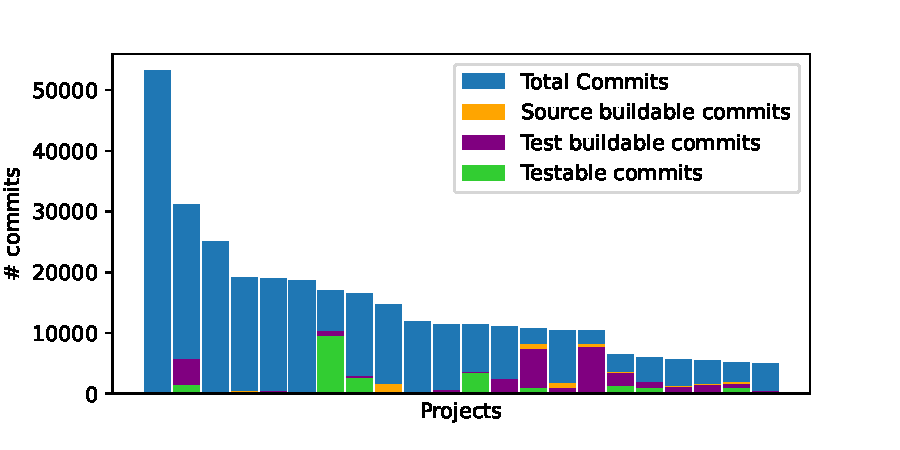
\includegraphics[width=0.8\textwidth]{pages/02-Testability/images/Many4j 1-22.pdf}
    \caption{Project metrics (Large projects)}
    \label{fig:many4j-1-bar-chart}
\end{figure}%
\begin{figure}[h!]
    \centering    
    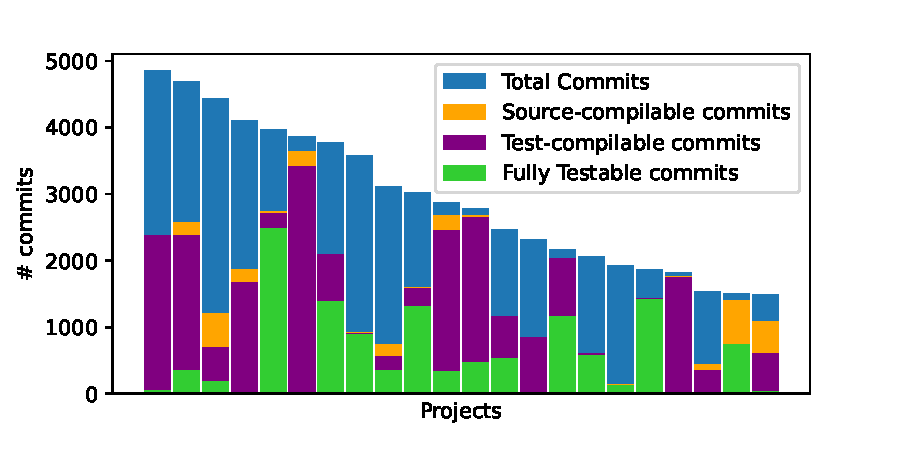
\includegraphics[width=0.8\textwidth]{pages/02-Testability/images/Many4j 23-44.pdf}
    \caption{Project metrics (Medium projects)}
    \label{fig:many4j-2-bar-chart}
\end{figure} 
\begin{figure}[h!]
    \centering    
    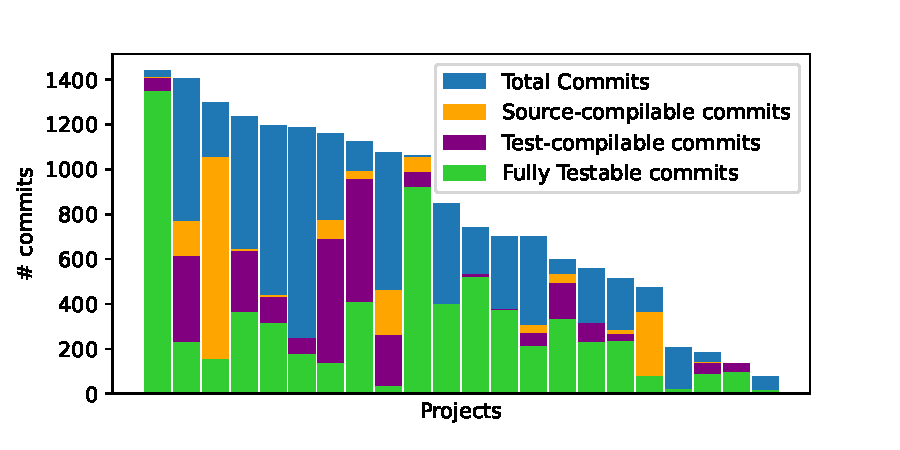
\includegraphics[width=0.8\textwidth]{pages/02-Testability/images/Many4j 45-66.pdf}
    \caption{Project metrics (Short projects)}
    \label{fig:many4j-3-bar-chart}
\end{figure}

\section{Analysis}
\label{sec:testability:analysis}
Let's now analyze in some more detail some \patxi{the} results presented in the previous section.

The mean \textbf{Source Compilability} of the projects (47.29\%), although low, is slightly higher than in previous studies on Java projects such as that of Tufano et al (38.13\%). 
This is partly due to having left out 20 projects whose compilability was 0.
But what is more interesting is the differences from project to project, something that was expected, and seen in previous studies on the matter~\cite{tufano2017there,sulir2020large,querel:2021:warning}.

The mean value of the \textbf{Test Compilability\textsubscript{A}} is significantly lower (41.73\%), because Source Compilability is a threshold for this metric.
Moreover, considering only those commits where the source code is compiled, the \textbf{Test Compilability\textsubscript{S}} offers a considerably higher value on average (88\%).
This value is reasonable, since once the main source code was built \patxi{compile?}, it is more likely that the test code can also be built\patxi{compile? Revisar todos los build y built}. 
% What is maybe unexpected, as we will discuss later in Section~\ref{sec:semantics}, is that it is not even higher.
We also note that for this metric, 50\% of the projects offer a value higher than 97\%.\patxi{Therefore, test compilation does not seem a problem in general, and efforts, in any case, should be put in source compilation.}


%In contrast, it seems that the compilability of both source code and tests is significantly lower than for projects collected through the GitHub API. Many4J projects offer a significantly lower mean on all parameters.

The most clear result when analyzing testability of projects is its variability from project to project. 
Figure~\ref{fig:testability-overview} illustrates this, by showing the shape of the distribution of all testability metrics we defined, for all projects.

\begin{figure*}[ht!]
    \centering    
    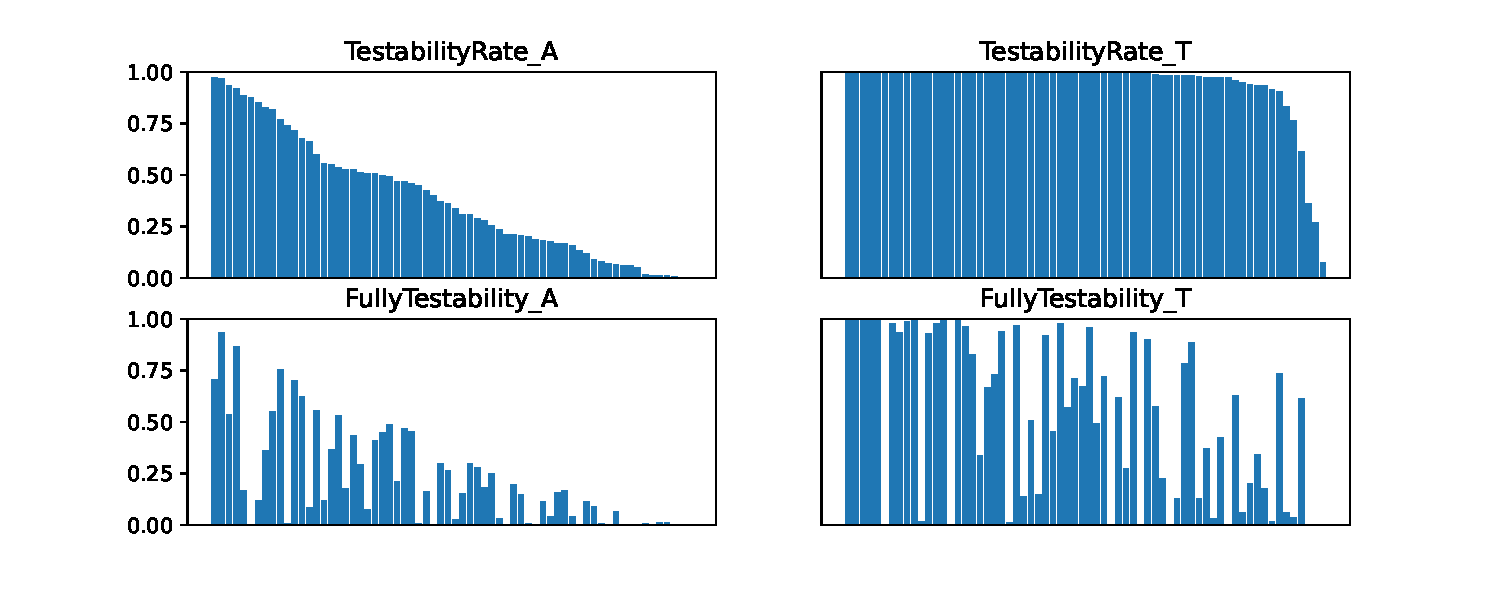
\includegraphics[width=\textwidth]{pages/02-Testability/images/Overview.pdf}
    \caption{Overview of testabilities - Each bar represents a project. Each column\patxi{column? Hay que ver cómo decir esto que se entienda mejor} is ordered by the corresponding Testability Rate (A and T) of each project.}
    \label{fig:testability-overview}
\end{figure*}

Looking at the Testability Rate values, when we focus on those commits where the tests can be built (\textbf{Testability Rate\textsubscript{T}}) we observe an average value of 94.14\%, a high percentage of the project's tests are executed successfully. 
% Again, we see that the \textbf{Testability Rate\textsubscript{T}}, as with other values, varies a lot between projects, with the median of this value being 99.53\%, indicating that in 50\% of the cases almost all the tests pass for test compilable commits.
By calculating the Testability Rate considering all commits (\textbf{Testability Rate\textsubscript{A}}), this value gives an overview of the testability of the project and how Source Compilability impacts running tests on past commits.

Focusing on \textbf{Fully Testability\textsubscript{T}}, we could expect it would be usually high: developers should write code that does not break \textit{all} the tests. 
Fact is that in more than half of the commits that were test-compilable some tests fail when they are run. 
This result, which may seem surprising, deserves as well more discussion that we will provide in Section~\ref{sec:low-testability}.\patxi{¿Por qué no aquí si estamos en la sección de análisis?}

\textbf{Fully Testability\textsubscript{A}} gives quite interesting information: the fraction of commits that are testable, with respect to the total number of commits. 
When compilability is low, this fraction is necessarily low, just meaning that commits are not testable because they are not source- or test-compilable. 
When compilability is high, \textit{Fully Testability\textsubscript{A}} really shows differences.\patxi{¿Qué diferencias¿Entre proyectos? -> among projects} 

With the data presented up to here, we can already answer RQ\textsubscript{1}, RQ\textsubscript{2} and RQ\textsubscript{3}\patxi{Ojo, la numeración de las RQs ha cambiado: 2.1, 2.2, 2.3, y en los siguientes párrafos igual}:

\vspace{0.5cm}
\fbox{\begin{minipage}{\textwidth}
\textbf{\textbf{RQ\textsubscript{1}}: ``\RQI''}
We found 93,925 test-compilable commits out of 103,097 source-compilable commits.
When calculating \textit{Test Compilability} using all the commits of the project we obtain an average value of 41.73\%, while if we compute only the commits in which we can compile the source code, the average value increases significantly (88.2\%).\patxi{Hay que aportar algo más aquí que sólo los datos. ¿Qué implica esto?: We can conclude that when the source code compiles, the test code compile, therefore, in general, test compilation is not an issue.}
\end{minipage}}

\vspace{0.5cm}
\fbox{\begin{minipage}{\textwidth}
\textbf{\textbf{RQ\textsubscript{2}}: ``\RQII''}
We found 40,540 fully-testable commits out of 93,925 test-compilable commits. 
When calculating \textit{Fully Testability} using all the commits of the project we obtain an average value of 22.12\%, while if we compute only the commits in which we can compile the tests, the average value increases significantly (52.53\%).\patxi{This is quite surprising, as one would expect that all tests should pass before a commit is accepted (after all, this is what CI is for). The results that we show here indicates that this is not always the case. We discuss it further in the next section.}
\end{minipage}}

\vspace{0.5cm}
\fbox{\begin{minipage}{\textwidth}
\textbf{\textbf{RQ\textsubscript{3}}: ``\RQIII''}
When calculating \textit{Testability Rate} using all the commits of the project we obtain an average value of 38.63\%, while if we compute only the commits in which we can compile the tests, the average value increases significantly (94.14\%).\patxi{This is in line with our expectations: in general when the tests compile, they succeed.}
\end{minipage}}
    


\section{Discussion}
\label{sec:testability:discussion}
After presenting the main results, and its analysis, in this section we discuss some details of our studies, including the threats to their validity.
%In conducting the different studies, we have found that there is a great variety in the testability of the different projects, even within the same study. In this section we will discuss the semantics of the testability metrics, analyse some of the projects with the higher testability, study why projects have low testability and, finally, present the  threats to validity of this work.

\michel{Aqui faltan dos subsecciones: una sobre la semantica de las metricas, y otra sobre los proyectos con alta testabilidad. La primera queda bastante obsoleta con el CaseStudy, la segunda tendría que volver a escribirla, ya que las métricas no son las mismas}

% \subsection{On the semantics of testability metrics}
% \label{sec:semantics}

% \michel{Es posible que esta sub-sección, con el nuevo Case Study, no tenga mucho sentido}

% For the studies presented in this paper, we designed a framework based on extending buildability to consider also buildability of tests, and introducing four \textit{Testability} metrics. 
% Each of these metrics shows a different aspect of testability.

% In continuous integration systems it is common that all tests must pass, being the result of their execution a binary value: either all tests pass or all tests fail. 
% In this context, we define that a commit is FullyTestable if all tests are success. 
% At the project level, we can identify how many commits are FullyTestable and provide a metric representing their percentage (Fully Testability). 
% It is common to consider all the commits of a project to calculate this type of metric.
% \textit{Fully Testability\textsubscript{A}} could be considered the ``absolute'' testability, since it considers all commits.
% In a project with 100\% \textit{Fully Testability\textsubscript{A}} all past snapshots are testable. 
% However, there are constraints, not related to the tests themselves, that put limits to testability.
% For example, a test that cannot be built, cannot be run. 
% Therefore, we defined \textit{Fully Testability\textsubscript{T}} to capture these constraints, and define testability related to them. 
% They inform on the quality of the tests only for snapshots that are buildable (either source- and tests-buildable). 
% In more detail:

% \begin{itemize}
%     \item \textbf{A high \textit{Fully Testability\textsubscript{A}}} signals a \textbf{highly reproducible project}: most of its snapshots are buildable, and the execution of their tests is successful.
%     The project in our dataset with the highest value in this metric is \textit{jsoup}, with a value of 93.55\%. 
%     This project, and others with high \textit{Fully Testability\textsubscript{A}}, are analyzed in the section~\ref{sec:high}.
%     \item \textbf{A high \textit{Fully Testability\textsubscript{T}}} hints to a project with \textbf{highly reproducible execution of tests}: most tests that can be built can also be executed successfully. 
%     A good example is \textit{JFinal}, with a value of 100\%. 
%     Its low \textit{Test Buildability} (22\%) considerably affects its \textit{Fully Testability\textsubscript{B}} (22\%). 
%     In this case, \textit{Fully Testability\textsubscript{T}} shows that as long as the tests are built correctly, they can be executed successfully. 
%     In projects with high \textit{Fully Testability\textsubscript{T}} and low \textit{Test Buildability} it is reasonable to think that improving \textit{Test Buildability} could increase also \textit{Fully Testability\textsubscript{A}}.
% \end{itemize}

% There are some projects as well with a high percentage of tests executed successfully, but low \textit{Fully Testability}. 
% This is possible when many tests in a snapshot are executed successfully, but a few do not. 
% For example, Figure~\ref{fig:checkstyle} shows a stacked area chart of the test results for all snapshots of \textit{Checkstyle}: snapshots are in the X axis, and the number of tests for each of them in the Y axis. Most of the tests for each snapshot are green (test success), but there is a small orange area close to the X axis corresponding to tests executed with error. 
% Due to these errors, most of the commits are not testable, and the project has a very low \textit{Fully Testability\textsubscript{A}} (1\%). 
% The reason for this is binary definition for Fully Testability, based on the rule of ``all tests should pass''. 
% Even when it is useful to compare with the ideal situation, there is room for defining additional metrics that reflect the high reproducibility of the tests in projects like this.

% \begin{figure}[t]
%     \centering    
%     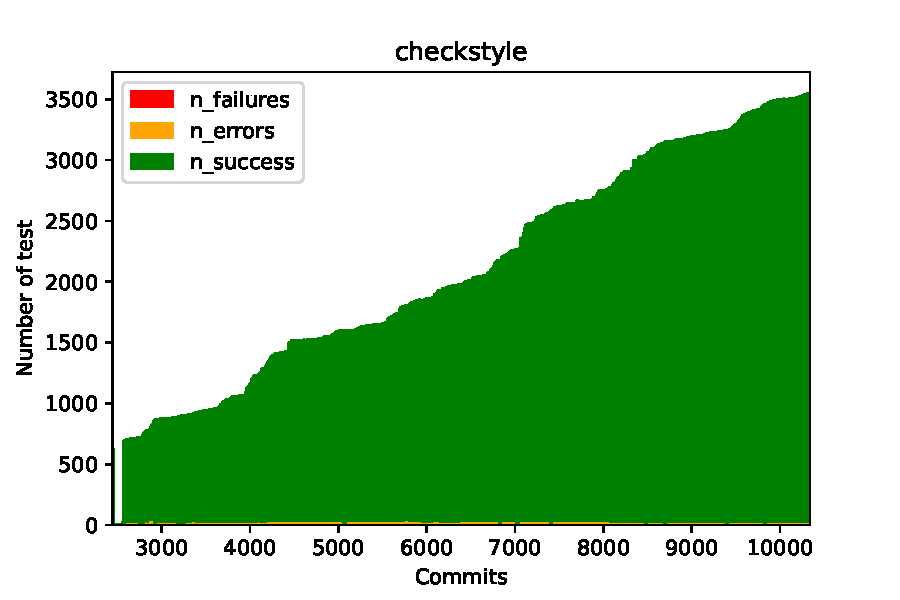
\includegraphics[width=8cm]{images/checkstyle.pdf}
%     \vspace{-0.2cm}
%     \caption{Tests results for Checkstyle project}
%     \label{fig:checkstyle}
% \end{figure}

% For this purpose, for each project commit, we define \textit{TestableRate}. 
% This value will show us the ratio of tests with a success result against the total number of tests of that commit. 
% In this way, \textit{TestableRate} gives us a more complete view of how the tests have behaved in a commit.
% Thus, a commit being \textit{FullyTestable} would only be a particular case where the value of \textit{TestableRate} is 100\%.

% In order to study the percentage of tests that pass at the project level, we find that it is difficult to capture in a metric that clearly reflects how the tests behave in the commit history. 
% The main limitation is when we consider all commits, since in those where the source code or test code cannot be built, we assume a TestableRate of 0\% because we do not know the real TestableRate.

% To illustrate it in an example, in Figure~\ref{fig:closure} we see the result of the tests in the history of the Closure project. 
% Several commits on its commit history cannot be built. 
% The mean TestableRate of all its commits is 59\%, while the median reaches 100\%.
% As in Fully Testability, in order to deal with the limitations of project buildability, Testability Rate C, B and T, considering all commits, source-buildable and test-buildable commits respectively, are defined in an analogous way.

% \begin{figure}[h]
%     \centering    
%     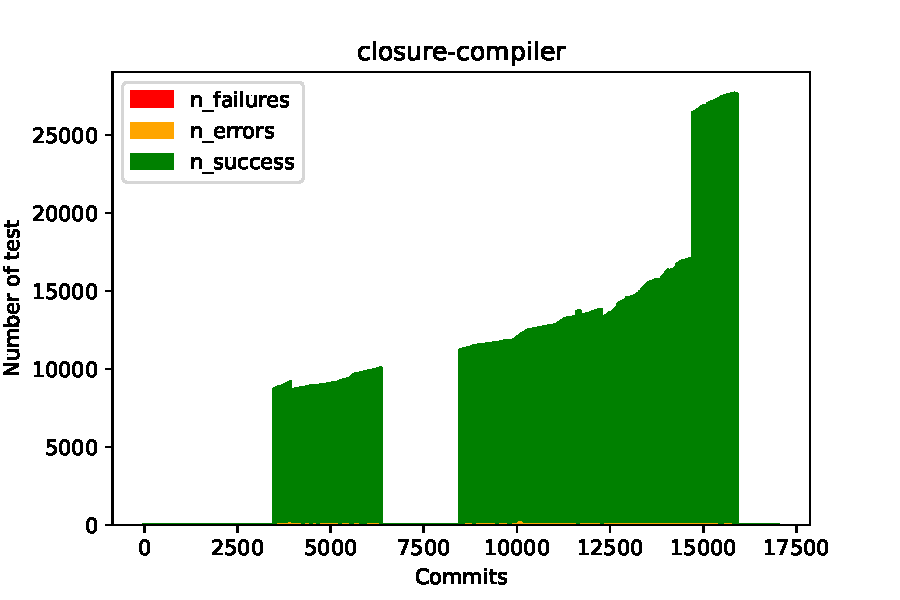
\includegraphics[width=8cm]{images/Closure.pdf}
%     \vspace{-0.2cm}
%     \caption{Tests results for Closure Compiler project}
%     \label{fig:closure}
% \end{figure}

% \subsection{Projects with high testability}
% \label{sec:high}

% We have identified some projects with high testability, which deserve a separate analysis. 
% To show these cases, we have searched for projects with the highest \textit{TestabilitRate} and the highest \textit{Fully Testability}.

% After analyzing the Testability Rate of the projects, we wanted to check which projects offer the highest results. Of the 86 projects:
% \begin{itemize}
%     \item We found 11 where the Testability Rate\textsubscript{A} is 100\% (i.e. in at least 50\% of their commits all the tests pass).
%     \item We found 39 where the Testability Rate\textsubscript{B} is 100\% (i.e. in at least 50\% of their source-buildable commits all the tests pass).
%     \item We found 44 where the Testability Rate\textsubscript{T} is 100\% (i.e. in at least 50\% of their test-buildable commits all the tests pass).
% \end{itemize}

% These values give us a very high number of projects, making an in-depth analysis difficult. 
% Therefore, in order to study projects with high testability, we have limited to those with high Fully Testability. 
% Specifically, we have selected the 3 projects that offer the best results for the different variants of Fully Testability (C, B and T).

% Tables~\ref{table:high-testability-A} and~\ref{table:high-testability-T} show metrics of the three projects with the highest Fully Testability of each flavor (A and T). 
% % La siguiente frase necesitaria más desarrollo
% %They could be good for identifying good practices that may help to increase testability of other projects.

% \begin{table}[h]
%     \centering
%     \caption{Top three projects with the highest \textit{Fully Testability\textsubscript{A}}}
%     \label{table:high-testability-A}
    
%     \begin{tabular}{|r|r|r|r|}
%         \hline
%         \textbf{Project}                  & \textbf{jsoup} & \textbf{spark} & \textbf{retrofit} \\ \hline
%         \textbf{Age}                      & 11.12          & 9.54           & 10.47         \\ \hline
%         \textbf{LoC}                      & 17,831         & 8,655          & 22,003           \\ \hline
%         \textbf{Total Commits}            & 1,442          & 1,062          & 1,865              \\ \hline
%         \textbf{Source buildable commits} & 1,410          & 1,051          & 1,431              \\ \hline
%         \textbf{Source buildability}      & 0.97           & 0.98           & 0.76          \\ \hline
%         \textbf{Test buildable commits}   & 1,403          & 986            & 1,431              \\ \hline
%         \textbf{Test buildability}        & 0.99           & 0.93           & 1.0               \\ \hline
%         \textbf{FullyTestable commits}    & 1349           & 921            & 1,411              \\ \hline
%         \textbf{Fully Testability\textsubscript{A}}      & \textbf{0.93} & \textbf{0.86} & \textbf{0.75} \\ \hline
%         \textbf{Fully Testability\textsubscript{B}}      & 0.95           & 0.87           & 0.98          \\ \hline
%         \textbf{Fully Testability\textsubscript{T}}      & 0.96           & 0.93           & 0.98          \\ \hline
%         \textbf{Testability Rate\textsubscript{A}}       & 1.0            & 1.0            & 1.0               \\ \hline
%         \textbf{Testability Rate\textsubscript{B}}       & 1.0            & 1.0            & 1.0               \\ \hline
%         \textbf{Testability Rate\textsubscript{T}}       & 1.0            & 1.0            & 1.0               \\ \hline
%     \end{tabular}
% \end{table}

% Among the projects with a high \textit{Fully Testability\textsubscript{A}} is \textit{jsoup}, a popular programming library for manipulating HTML code, which has only unit and integration tests.
% The second project, \textit{retrofit}, is a simple HTTP client, with the particularity that it is a multi-module project. 
% A high t\textit{Fully Testability\textsubscript{A}} C indicates that the tests of all its modules pass completely in most of the commits.
% All its tests use mocks, defined in its own module. 
% The robustness of testing functionality with mocks rather than with real endpoints (subject to change over time) may be one of the reasons for the good results of this project in this metric.
% The third project, \textit{spark}, is a lightweight web development framework. 
% It has end-to-end tests to verify the correct behavior when HTTP requests are performed; we have observed that these requests do not depend on remote services, though, which we have found in other projects to be a reason for low testability (see Section~\ref{sec:low-testability}).

% \begin{table}[h]
%     \centering
%     \caption{Top three projects with the highest \textit{Fully Testability\textsubscript{T}}}
%     \label{table:high-testability-T}
%     \begin{tabular}{|r|r|r|r|}
%         \hline
%         \textbf{Project}                  & \textbf{otto} & \textbf{javapoet} & \textbf{camel} \\ \hline
%         \textbf{Age}                      & 5.85          & 8.88              & 14.28          \\ \hline
%         \textbf{LoC}                      & 1,344        & 8,306            & 1,146,447      \\ \hline
%         \textbf{Total Commits}            & 205           & 846               & 53,286          \\ \hline
%         \textbf{Source buildable commits} & 18            & 398               & 21             \\ \hline
%         \textbf{Source buildability}      & 0.09          & 0.47              & 0.0            \\ \hline
%         \textbf{Test buildable commits}   & 18            & 396               & 20             \\ \hline
%         \textbf{Test buildability}        & 1.0           & 0.99              & 0.95           \\ \hline
%         \textbf{Fully Testable commits}   & 18            & 396               & 20             \\ \hline
%         \textbf{Fully Testability\textsubscript{A}}      & 0.09          & 0.47              & 0.0            \\ \hline
%         \textbf{Fully Testability\textsubscript{B}}      & 1.0           & 0.99              & 0.95           \\ \hline
%         \textbf{Fully Testability\textsubscript{T}}      & \textbf{1.0}  & \textbf{1.0}      & \textbf{1.0}   \\ \hline
%         \textbf{Testability Rate\textsubscript{A}}       & 0.0           & 0.0               & 0.0            \\ \hline
%         \textbf{Testability Rate\textsubscript{B}}       & 1.0           & 1.0               & 1.0            \\ \hline
%         \textbf{Testability Rate\textsubscript{T}}       & 1.0           & 1.0               & 1.0            \\ \hline
%     \end{tabular}
% \end{table}

% The three projects selected for the table with the highest \textit{Fully Testability\textsubscript{T}} are particularly interesting: whenever their tests could be constructed, they could be executed successfully. Two of them appeared in previous tables (\textit{otto} and \textit{javapoet}). The \textit{camel} project (a service integration library) offers a high \textit{Fully Testability\textsubscript{T}}, but this result must be considered in view of the fact that its buildability is only 0.03\%. For projects like this it is important to consider all \textit{Fully Testability} variants. 

\subsection{Why do projects have low testability?}
\label{sec:low-testability}

We have performed a preliminary study to identify the main reasons for some projects having low Fully Testability\textsubscript{A}. 
These reasons can be organized in three types:

\subsubsection{Low buildability.} 

\textit{Fully Testability\textsubscript{A}} of a project depends on the steps prior to the execution of the tests: building the main source code and the tests.
In projects with low buildability, testability is constrained by it.
Tufano et al. showed how one of the main reasons why a commit is no longer buildable is because of an error in obtaining the project dependencies~\cite{tufano2017there}. 
Therefore, it is possible that if those dependencies were available, the project not only built correctly, but also its tests could be executed successfully. 
We found several projects where the \textit{Fully Testability\textsubscript{A}} is low due to low buildability, but \textit{Fully Testability\textsubscript{B}} and \textit{Fully Testability\textsubscript{T}} are high.

\subsubsection{Snapshots were never testable.} When the project was being developed, not all of its commits were testable:

\begin{itemize}
    \item  \textbf{No tests in the snapshot}: 
    In some projects we have found no tests. 
    We consider these commits without test as non-testable, resulting in low values if many snapshots are like that.
    In these cases, maybe the project has tests, but they are not in the Maven project.
    \item \textbf{Snapshots with tests failing}: 
    When building and running tests on snapshots, we decided to try all of them in the master branch, since a recent study by Kovalenko et al.~\cite{kovalenko:2018:miningfilehistories} has shown that considering additional branches does not seem to have a significant impact compared to using only the master branch. 
    But depending on the strategy used by the developers to merge changes into master, we may find commits with tests failing even when they were merged. 
    For example, a commit includes a new feature which breaks some tests, but it is still merged, maybe because the next commit will fix the tests or the cause of the error.
    We found this case in \textit{elastic-job} by taking advantage of commit comments to understand the development workflow. 
    When refactoring, tests stop passing in some commits, being fixed in later commits (for example see commits 860, 929, 965, 1053 and 1120, where 0 is the last commit in the history).
    So, if some tests of a project were never testable, it is not possible to make the snapshot testable when reproducing the past.
\end{itemize}

\subsubsection{Context is not reproduced.} 
Without the right context, some tests cannot perform exactly as they did in the past. Here are some of the problems related to test execution context:

\begin{itemize}
    \item \textbf{Network services}: 
    In most of the integration test, the tests check how the software integrates with other network services. If these services need to be launched prior to running the tests, we will find connection-related exceptions when running the tests without the network services.
    A good example is the \textit{Jedis} project: it is a library for managing a Redis database. 
    If this database has not been launched when running the tests, the tests throw exceptions such as ``ConnectException'' or ``ConnectionRefused''.
    To address this type of problem, a good practice would be for the test itself to be able to launch the necessary context to be able to be executed.
    \item \textbf{Command line tools}: 
    There are tests that require command line tools like Python, Perl or G++ to be executed successfully. 
    The \textit{antlr4} project has failed tests in the absence of these services. 
    For example, this project requires in different commits different versions of Python (2.7 or 3.5).
    \item \textbf{System resources}: 
    Some projects require access to certain system resources for their tests. 
    For example, the \textit{Activiti} and \textit{FastJSON} projects require access to font-related resources (through the \texttt{SunFontManager} and \texttt{X11FontManager} classes respectively). 
    The experiments have been run on machines that do not have a GUI and therefore these resources are not part of the system.
    \item \textbf{Remote resources}: 
    There are tests that require accessing remote services and making requests on them. 
    If these resources have changed or are no longer accessible, they compromise the test results. 
    We found an example in the \textit{checkstyle} project, where an attempt is made to download an XML file and parse it, failing in this last step, probably because it has been modified over time.
    This type of bugs has been characterized as \textit{extrinsic}~\cite{rodriguez2020bugs,rodriguezperez2020watch,rodriguez2018if}, since the problem is not in the source code, but in an external service.
    \item \textbf{Reflection}: 
    In Java it is possible to load classes through reflection. 
    These classes have not been checked by the compiler in the construction phase of the tests, so in case of error or absence of the class, the error appears at test runtime. 
    An example of this case can be found in the \textit{Okhttp} project, where we found the ``Could not initialize class SSLExtension'' error, being a class loaded by reflection.
    In detail, the class is not available because although a supported version of Java is used, the JDK distribution used does not have such a class.
\end{itemize}

So, when we find a non-testable snapshot, a question arises: Is it non-testable because it was originally non-testable, or because we cannot reproduce the test execution context properly?
If a project had a continuous integration (CI) system where tests are executed on every snapshot, we could answer the question by analyzing the test results in CI logs. Unfortunately, it is usual to remove CI logs frequently to save storage space. 
However, although having this information could be useful, not all of the cases above could be solved by improving the context of test execution. 
For example, we have no chance when working with remote resources over which we have no control.
Even so, the CI configuration files can provide information about how to reproduce the test execution context.
It remains as future work to explore this line to improve project testability when the test context is not properly reproduced. 

%We consider that the way of building and executing the tests carried out follows the standards of the technology used (Maven), which allows us to carry out an automatic analysis of buildability and testability.

\subsection{Threats to validity}

Our results are subject to construct validity issues, mostly due to how we define testability of a project: as the median percentage of test success with respect to the total and as percent of snapshots in which tests could be successfully executed). 
As we have shown, testability can have different values depending on which sample of snapshots is selected to define 100\% (all, source-buildable or test-buildable). 
It could be possible that in some cases our testability metrics hide the real behavior of the project in this respect.

Results are also subject to internal validity issues. 
For example, without the environment where the tests were originally run, they may give a different result (lack of libraries, binaries or specific configurations). 
They are also subject to any possible bug in our extraction and analysis tool. 
Therefore, all results together with the tools used are available in the reproduction package for inspection.

Finally, we can also have external validity issues. 
The dataset is composed only projects written in Java and most of their test are unit test, so the conclusions drawn may not be transferable to other programming languages or types of tests. 
Extension to other languages is still a matter of further research.


% \section{Conclusions}
% \label{sec:testability:conclusions}
% In this paper we have started a path to analyze to which extent past snapshots of a project can be tested. 
For that, we have conducted an empirical analysis of a large number of Java projects from a well-known dataset. 
We also propose a framework for conducting further analysis, based on the different steps needed to successfully run tests for each snapshot. 
Using this framework, we have found that for more than half the snapshots, all tests cannot be run successfully.
However, the main result is the high variability of testability from project to project, even within relatively homogeneous dataset. 
% In this respect, we also discard some hypothesis on the influence of characteristics of projects (lines of code, number of commits, age) in testability.

%In this paper we offer a study of the testability of the history of 111 Java projects, which extends previous studies on the buildability of project history. 
%We also provide a complete study that discards some of the most common metrics of a project (lines of code, number of commits or its age) as factors that determine its testability. 
%We have found that in most projects it is not possible to reproduce the tests in the past.
%In addition, we conducted a preliminary study of the causes that can lead to low testability in Java projects.
%Analysing the projects we have found great variability, even among projects selected under the same criteria. 

We note that many projects cannot rely on running tests in past commits, as these won’t run or even compile.
Testing snapshots of the past is fundamental for the maintainability of old versions of the project which are still in production. 
Therefore we expect more research in this area in the future. 
Fortunately, we have found some signals showing that good practices can be identified to increment testability of current snapshots (that will become past snapshots with time). 
We have also suggested some ways of increasing testability of past snapshots improving the methods we are using for building and running tests in them. Of course, extending our study to other samples of Java code, and to other programming languages, will improve our knowledge in this area.

%and also that some techniques could be used to of those snapshots, 
%Replication testing is essential to improve the maintainability of projects that need to be maintained in previous versions.
%Reproducing this study using other languages such as Python, Javascript or C++ could lead to interesting future work.

\section*{Reproducibility}
\label{sec:testability:repro}

A documented reproduction package is available\footnote{\url{https://github.com/BuildabilityResearcher/TestabilityStudy}}. 
It includes a link to an extra package in Zenodo (due to size limitations in GitHub), with raw results and a copy of all the git repositories at the time of the analysis.